% Required for inserting images

\documentclass[11pt]{article}%
% \usepackage[conf]{ametsoc}  
\usepackage{graphicx}
\usepackage{amsmath}
\usepackage{amsfonts}
\usepackage{amssymb}
\usepackage{fullpage}
\usepackage{tabularx}
\usepackage{subcaption}
\usepackage{booktabs}
\usepackage{appendix}
\usepackage{url}%
\usepackage{tikz}
\setcounter{MaxMatrixCols}{30}
\setlength{\parindent}{0pt}
\setlength{\parskip}{1em}
%TCIDATA{OutputFilter=latex2.dll}
%TCIDATA{Version=5.50.0.2960}
%TCIDATA{LastRevised=Thursday, May 23, 2024 18:43:32}
%TCIDATA{<META NAME="GraphicsSave" CONTENT="32">}
%TCIDATA{<META NAME="SaveForMode" CONTENT="1">}
%TCIDATA{BibliographyScheme=Manual}
%BeginMSIPreambleData
\providecommand{\U}[1]{\protect\rule{.1in}{.1in}}
%EndMSIPreambleData
\begin{document}
\title{DRAFT - July 8th - Custom Loss Functions in Fuel Moisture Modeling}
\author{
    \begin{tabular}[t]{c}
        Jonathon Hirschi \\
        University of Colorado Denver \\
        \\
        Advisor: Jan Mandel
    \end{tabular}
}

\date{Summer 2024}
\maketitle

\begin{abstract}
Fuel moisture content (FMC) is a key predictor of predicting wildfire rate of spread (ROS). Machine learning models of FMC are being used more in recent years, augmenting or replacing traditional physics-based approaches. Wildfire rate of spread (ROS) has a highly nonlinear relationship with FMC, where small differences in dry fuels lead to large differences in ROS. In this study, custom loss functions that place more weight on dry fuels were examined with a variety of machine learning models of FMC. The models were evaluated with a spatiotemporal cross-validation procedure to examine whether the custom loss functions led to more accurate forecasts of ROS. Results show that the custom loss functions improved accuracy for ROS forecasts by a small amount. Further research would be needed to establish whether the improvement in ROS forecasts leads to more accurate real-time wildfire simulations.
\end{abstract}

% Abbreviations section
\subsection*{Key Terms \& Abbreviations}
\begin{itemize}
    \item \textbf{FMC:} Fuel Moisture Content, a ratio interpretable as a percentage of the weight of water in a stick relative to the weight of the stick.
    \item \textbf{ROS:} Fire Rate of Spread, units of meters per second.
    \item \textbf{Response Variable:} the variable that is being modeled, or the output of the model.
    \item \textbf{Predictors:} data variables used to predict the response variable. Also known as features, covariates, etc.
    \item \textbf{Residual:} the difference between the predicted values of a model and the observed response value.
\end{itemize}


\newpage
\tableofcontents
\newpage

\section{Background}
\subsection{Wildfires \& Climate Change}

Wildfires impact our lives in many ways, including direct destruction from fires and other public health effects. Toxic gases and harmful particulate matter make wildfires a threat to air quality and human health as a result \cite{WHO-2024-WFS}. Wildfires also affect water quality by depositing metals and other toxins into waterways and contributing to erosion and flooding \cite{USGS-2024-WQA}. The U.S. Congress Joint Economic Committee estimated that total monetary costs of wildfires is between \$394 billion and \$893 billion after accounting for affects of burned structures, smoke impacts, watershed damage, etc. \cite{JEC-2023-CEW}.

There are complicated interactions between the environment, human activity, and wildfires. Some important weather patterns make fires more prevalent and more severe when they do ignite. Drought is considered the “dominant driver of fire emissions” \cite{IPCC-2021-LCI} because dry vegetation provides the needed fuel for fires. Both the lack of precipitation and lower air humidity contribute to dry fuels. Wind is another key factor in fire activity. Strong winds dry out fuels, making fires more likely to ignite, and once fires are underway wind feeds the fire oxygen and physically spreads the flames, thus increasing wildfire spread \cite{Richardson-2022-GIW}.

Climate change is projected to increase the frequency and severity of wildfires, caused primarily by higher temperatures and less frequent precipitation. There is clear evidence that the changes predicted by climate models are already underway. The total burned area has increased, and more areas of the world are susceptible to fires \cite{IPCC-2021-LCI}. The three largest fires in Colorado’s history all occurred in 2020 \cite{CDFPC-2024-HWI}. Wildfires are also more frequent overall and more common throughout the year, even during months that traditionally were wetter and less prone to ignition. The IPCC  reports that “fire weather season has already lengthened by 18.7\% globally between 1979 and 2013” \cite{IPCC-2021-LCI}. Traditionally, the months of May through September were considered Colorado’s fire season \cite{WFCA-2023-CFS}. However, the most destructive wildfire in Colorado’s history, the Marshall Fire, occurred outside of Boulder in December of 2021. \cite{CDFPC-2024-HWI} 


\subsection{Fuel Moisture Content}

Fuel moisture content (FMC) is a critical component of wildfire susceptibility and fire spread. It is a measure of the water content in vegetation, and is expressed as a percentage of the ``dry weight" of the fuel. \cite{NCEI-2024-DFM} The dry weight is what the fuel would weigh when entirely dried out. In practice, sticks of wood are dried out in kilns and weighed to determine the dry weight. An FMC of 0\% would be completely dry fuel, and FMC values can range over 100\% if the total weight of the water is greater than the dry weight of the plant material. The formula for FMC is:

\begin{equation}
    \text{FMC} (\%) = \frac{\text{Fuel Weight} - \text{Dry Weight}}{\text{Dry Weight}} \cdot 100\%
\end{equation}

Dry fuels burn more readily, and wetter fuels burn more slowly or not at all. Atmospheric conditions affect FMC in a variety of ways. Temperature is a key component of FM; warmer temperatures dry out fuels, with other factors being held constant. Relative humidity (RH) is another key component of FM; more moisture in the air generally leads to more moisture in fuels. Higher wind speeds lead to drier fuels. Finally, solar radiation dries out fuels. Cloudy days with little direct solar radiation will generally lead to higher FMC conditions \cite{NWCG-FireWeather}. It is important to note that these atmospheric conditions relate to each other in complicated ways. For example, higher temperatures can cause lower RH and are also associated with stronger solar radiation, all of which lead to lower FM. However, higher temperatures can cause more evaporation and lead to increases in precipitation, which in turn increases FM. 

Researchers typically model dead FMC, or the water content of dead vegetation, separately from the FMC of living plants.\footnote{In practice, the dead FMC models are used as an input into the live FMC forecasts. In WRF-SFIRE and elsewhere, the dead FMC model is adjusted to provide estimates of live FMC based on biological factors of the plant.} This is due to several factors. Living plants try to maintain homeostasis, so they resist large fluctuations in moisture caused by atmospheric conditions. The water content of dead fuel, on the other hand, responds readily to atmospheric conditions and therefore there can be large fluctuations that are relevant to wildfire spread. Additionally, live fuels are thought of as composites of various fuel types. A sagebrush, for example, has woody material of various diameters as well as herbaceous material. These various materials retain moisture in different ways and respond to fire differently \cite{NWCG-FireWeather}. In this project, only dead fuel moisture will be considered. 

Dead fuel moisture is divided into different classes based on how quickly the material responds to changes in atmospheric conditions. These include 1-hour, 10-hour, 100-hour, and 1,000-hour fuels \cite{NCEI-2024-DFM}. A 1-hour fuel, very small twigs for example, will get wetter quickly when exposed to precipitation, while a 1,000-hour fuel, such as a fallen log, would take much longer to absorb precipitation and thus the FMC changes slower. The classes are defined by the lag time which determines how quickly the fuel responds to a change in atmospheric conditions. A 10-hour class fuel approaches the equilibrium as $\exp(-t/10)$, where $t$ is the time in hours.

The National Interagency Fire Center (NIFC) operates Remote Automatic Weather Stations (RAWS) across the country to measure hourly FMC and other associated environmental variables \cite{NIFC-2024-RAW}. Figure \ref{fig:wfas_raws} shows the location of all RAWS with FMC sensors.

\begin{figure}[ht]
    \centering
    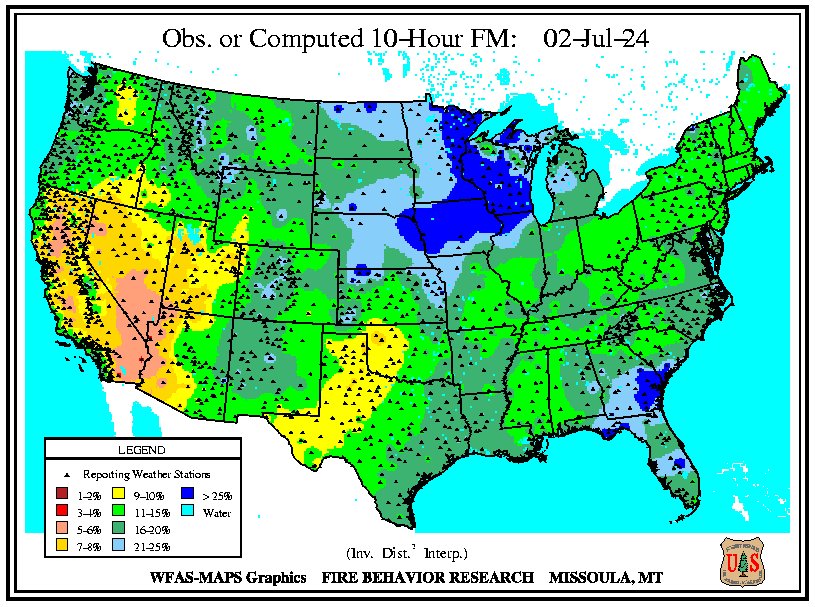
\includegraphics[width=0.8\textwidth]{images/WFAS-RAWS-map.png}
    \caption{All RAWS FMC locations.}
    \label{fig:wfas_raws}
\end{figure}

These RAWS stations\footnote{The ``S" in RAWS stands for station, so this is redundant terminology. It is an aesthetic preference that this terminology is more clear.} have sensors for 10-hour fuels, which consist of a 1/2 inch pine dowel with a moisture probe inside of it \cite{Campbell-2017-RMM}. Observations of 1-hour or 100-hour fuels are typically done through field observations. But for real-time FMC modeling, 10-hour fuels are the only type of fuel moisture with substantial data availability. In this project, dead 10-hour fuels will be examined for these reasons.

An important concept in FMC modeling is ``equilibrium moisture content". Theoretically, if environmental conditions are kept stable for a long period of time, the FMC of wood will equilibrate to its surroundings. The equilibrium FMC is the theoretical value that the FMC would approach over time, and it is calculated from relative humidity and temperature \cite{Mitchell-2018-CEM}. There are slightly different physical processes when fuels dry out or get wet, so researchers have developed the ``wetting equilibrium" and ``drying equilibrium" to establish what the equilibrium moisture content is for fuels under these two different scenarios \cite{Mandel-2014-RAA}. These variables are constructed from relative humidity (RH) and temperature\footnote{Units of degrees Kelvin.} (temp) in the following formulas:



\begin{equation}
\label{eq:equil}
\begin{split}
\text{Wetting Equilibrium} = &0.924\cdot\text{rh}^{0.679} + 0.000499\cdot\exp(0.1\cdot\text{rh}) + \\ &0.18\cdot(21.1 + 273.15 - \text{temp})\cdot(1 - \exp(-0.115\cdot\text{rh})) \\
\text{Drying Equilibrium} = &0.618\cdot\text{rh}^{0.753} + 0.000454\cdot\exp(0.1\cdot\text{rh}) + \\ &0.18\cdot(21.1 + 273.15 - \text{temp})\cdot(1 - \exp(-0.115\cdot\text{rh}))
\end{split}
\end{equation}

\subsection{Wildfire Rate of Spread}

The rate of spread (ROS) of a fire is a measure of how quickly fire propogates from a point of origin \cite{NFSC-2024-MFB}. Traditionally, this was measured in chains per hour, but in recent years researchers use the units meters per second. Factors affecting ROS include wind speed \& direction, fuel density and type (e.g. fine twigs versus big logs), and FMC. 

Figures \ref{fig:ros_other} and \ref{fig:fmc_ros_fmc} shows the idealized relationships between ROS and some other factors, while holding all else constant. These are model outputs from the physics-based tools within WRF-SFIRE. In this project, the idealized relationship for a category of fuel known as ``closed timber litter" will be used, since it is the most representative of the RAWS fuel moisture sensors of the available fuel categories developed by Anderson 1982. \cite{NIFC-2024-FAF} Figure \ref{fig:ros_other} shows the relationship between ROS and two key predictors: terrain slope\footnote{The units in this plot are tangent of the slope in degrees, so a value of 1 corresponds to $\text{tan} (45^\circ) = 1$} and wind speed. \cite{OpenWFM-2024-HTD} The relationship is approximately linear in both cases.


\begin{figure}[ht]
    \centering
    \begin{subfigure}{0.45\textwidth}
        \centering
        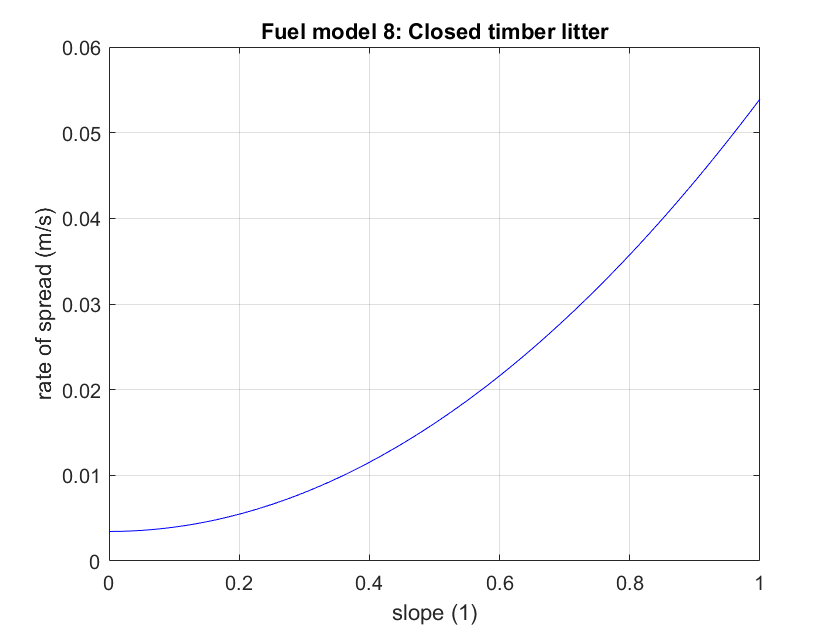
\includegraphics[width=\linewidth]{images/fuel8_ros_slope.png}
    \end{subfigure}
    \hfill
    \begin{subfigure}{0.45\textwidth}
        \centering
        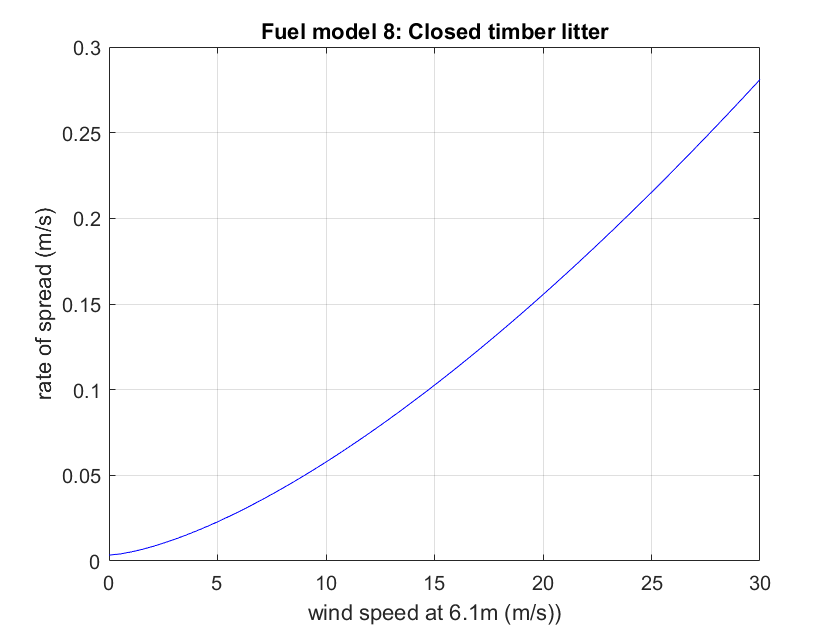
\includegraphics[width=\linewidth]{images/fuel8_ros_wind.png}
    \end{subfigure}
    \caption{ROS vs Slope and ROS vs Wind}
    \label{fig:ros_other}
\end{figure}


The relationship between ROS and FMC, however, is highly nonlinear, as seen in Figure \ref{fig:fmc_ros_fmc}. Small differences in the dry region of the plot, from 0\% to around 5\%, lead to very large changes in the resulting ROS. For the wetter region of the plot, the relationship with ROS is approximately flat until it reaches a ``moisture of extinction", where fire will not spread at all. This nonlinear relationship is of primary interest in this research project. 

\begin{figure}[ht]
    \centering
    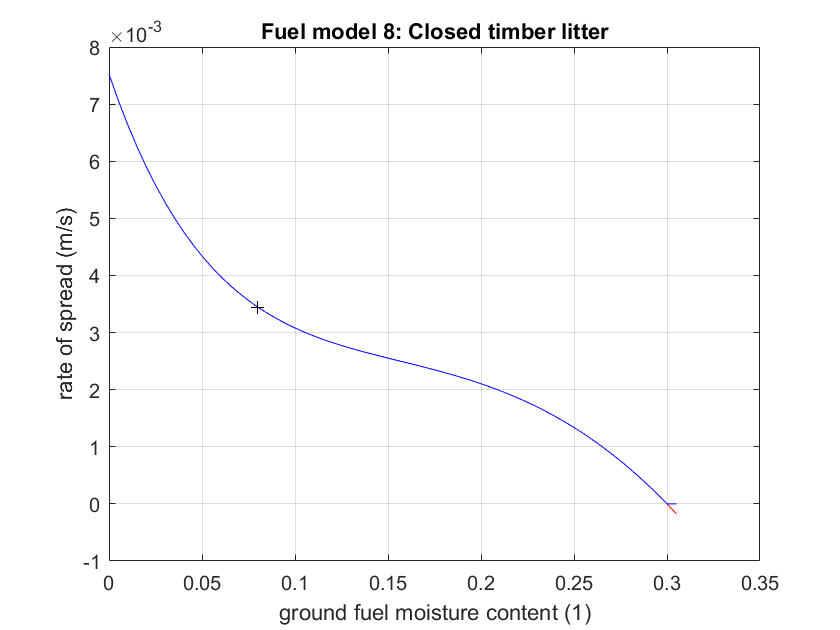
\includegraphics[width=0.8\textwidth]{images/fuel8_ros_fm.png}
    \caption{ROS vs FMC relationship.}
    \label{fig:fmc_ros_fmc}
\end{figure}

\subsection{Fuel Moisture Modeling}
\subsubsection{History \& Physics-based Methods}

Rothermel in 1972 developed a mathematical model of wildfire spread, based on physical properties of heat transfer, that included fuel moisture as one of the key parameters \cite{Rothermel-1972-MMP}. This model has been used and built upon by wildfire researchers for decades. 

WRF-SFIRE is a real-time forecasting project for wildfires which combines an extensive set of mathematical methods and data processing techniques \cite{OpenWFM-2024-HTD}. Within WRF-SFIRE, there is a physical model of FMC developed by Mandel (2014), which uses theoretical physical properties of wetting and drying, combined with data assimilation through the augmented Kalman filter \cite{Mandel-2014-RAA}. The core differential equation in the model uses wetting equilibrium moisture, drying equilibrium moisture, and precipitation and as data inputs.

Many other physics-based models of FMC have been developed. All use some combination of relative humidity, temperature, \& precipitation to estimate FMC from physical principles, and typically field observations of FMC are used to tune parameters. \cite{Catchpole-1999-EFR,Nelson-2000-PDC, vanderKamp-2017-MFS}

\subsubsection{Machine Learning models of FMC}

With modern advances in computing and more extensive observed FMC data, machine learning models of FMC have become more popular. Machine learning is a general term for statistical models that are trained on observed data and used to predict new, unobserved data. The models researchers have considered have commonly included some form of linear regression, random forests, or XGBoost.\footnote{See Methods section for more detail on these model architectures.} These models are not recursive\footnote{A recursive model in this sense is any that models the FMC at a given time as a function of the FMC at previous times.} in time, meaning that the models are mapping observed weather conditions to the response variable of FMC at each instance of time without explicitly including a temporal relationship.\footnote{Using derived time predictors like hour of the day and day of the year can help a model learn some time dependence, but this is different than a recursive model like autoregression or a Recurrent Neural Network (RNN).} 


Using the previously mentioned machine learning models, without explicit time recursion, is an active area of research in the fuel moisture modeling literature. Lee 2020 fit various statistical models to ground station observations in South Korea, and selected a Random Forest model as the most accurate. \cite{Lee-2020-EFM} Researchers at the National Center for Atmospheric Research (NCAR) conducted a larger study in the United States by developing and evaluated a number of machine learning models of FMC using weather data from the HRRR weather model and NASA's VIIRS satellites \cite{McCandless-2020-EWS, Schreck-2023-MLV}. The final model in their publicly available 10-hour FMC forecasting tool is an XGBoost. 

Physics-based models of FMC are time-dependent differential equations, so they are recursive in this way. The underlying physical process is time dependent, so an active area of research is to use temporally recursive models for fuel moisture modeling. Kang 2022 test autoregressive models and a LSTM\footnote{Long Short Term Memory, a variety of recurrent neural networks specialized for time series.} to predict monthly averaged FMC observations. \cite{Kang-2022-FMC} Other recent efforts to use recurrent neural networks (RNNs) include Fan 2021, where an LSTM was built with the 2017 Vanderkamp physical model of FMC as an input \cite{Fan-2021-PGD}. There is not a widely available FMC model product built on recursive machine learning models at this time.


\subsection{Loss Functions in Machine Learning}

\subsubsection{Loss Functions Overview}

A loss function is intended to measure the fitting accuracy of a statistical model. Loss functions are used for training the parameters machine learning models. Model parameters are chosen by minimizing the loss function. This can be done analytically for models like linear regression, but for more complicated models it must be estimated using some variety of gradient descent. 

When the response variable is continuous, as is the case with modeling FMC, the standard choice of loss function is the mean squared error (MSE), which is equivalent to the L2 norm of the vector of model residuals. Suppose there is an observed vector of response data $y$ of length $N$ and a vector of model predictions $\hat y$. The $i^{th}$ residual of the model would be $(y_i - \hat y_i)$. The MSE for the model would thus be:


\begin{equation}
    \label{eq:mse}
    \text{MSE} = \frac{1}{N}\sum_{i=1}^N r_i^2 = \|r\|_2^2
\end{equation}

There are many other potential loss functions for continuous data, such as the the mean absolute error, equivalent to the L1 norm of the residuals. In this project, a number of weighted MSE loss functions will be considered. Weighted least squares minimizes the weighted residual sum of squares, with a weight $w_i$ applied to each residual value.\footnote{It is not strictly required for the weights to sum up to 1. In many machine learning contexts, scaling the weights so that they sum to 1 leads to identical results.}


\begin{equation}
    \label{eq:wmse}
    \text{Weighted MSE} = \frac{1}{N}\sum_{i=1}^N w_i\cdot r_i^2
\end{equation}

Weighting the loss function introduces bias into the estimator when considering the accuracy of the predictions. This addition of bias can be beneficial if the variance of the estimator is sufficiently reduced. This dynamic is referred to as the ``bias-variance tradeoff" (CITE ESL pg 37). Weighted loss functions have been most commonly used in the context of classification problems. \footnote{The loss function for a classification problem would not be MSE, but rather something like cross-entropy which is intended for categorical model output.} When trying to build classification models on highly imbalanced datasets, such as when predicting a very rare disease, it is often desirable to weight the loss function to give more weight to the underrepresented class. For example, in a model of a rare disease where only 1 out of 1 million observed people has the disease, a model could correctly predict 999,999 out of 1 million cases correctly by predicting that nobody has the disease. The model will of course never correctly predict that somebody has the disease, so this is undesirable behavior. Weighting the loss function so that the rare cases contribute more to the total model loss can control for these errors. With continuous response variables, weighted loss functions are used for outlier detection, where iterative schemes identify influential observations and downweight them so they do not have an outsize effect on the final model fit. This is the technique used in various robust regression algorithms.\cite{OLeary-1990-RRC} In this project, weighted MSE loss functions with a continuous response variable will be considered based on purely physical considerations of the problem, not meant to address any outlier issues. 

\subsubsection{Custom Loss Functions in Environmental Science}

Within wildfire modeling and broader environmental science literature, custom loss functions have been used in a number of studies, but primarily for imbalanced classification tasks as discussed previously. Researchers from the Cooperative Institute for Research in the Atmosphere (CIRA) at Colorado State University published a guide to implementing custom loss functions for environmental science applications in 2021, with a number of applications related to storm detection, generating synthetic radar imagery, and more. \cite{Ebert-2021-GCL} The paper introduces a simple exponentially weighted loss function\footnote{\cite{Ebert-2021-GCL} at Page 7.}, which will be used in this project, along with instructions to implement these loss functions in the Tensorflow software library for neural networks.

Detecting wildfires using remote sensing is an active area of research, and machine learning methods of image processing are popular. The problem is often framed as a classification task, where given a grid of pixels in a image, the model classifies each pixel as fire or not fire. Since the goal is early detection of wildfires, when there are fires present the number of fire pixels is very small relative to the overall number of pixels in the image. Thus, this is an imbalanced classification task and weighted loss functions are useful. Yang 2021 and Pande 2021 both use variations of convolutional neural networks for classification with weighted loss functions to address class imbalance \cite{Yang-2021-PFF}\cite{Pande-2021-WSF}.

In a slightly related project, Buch 2022 use a variety of neural network to predict wildfire frequency and burned area in the Western US \cite{Buch-2022-SML}. A custom loss function is used to get the network to minimize the loss over a statistical distribution, rather than minimizing the loss for a single output of the model.

For weighted loss functions specifically related to modeling FMC, researchers have used weighted loss functions when investigating the relationship between FMC and soil moisture. Lu 2021 use a robust regression procedure to downweight influential observations when using satellite observations to model soil moisture and live FMC. \cite{Lu-2021-EMS} Rakmatulina 2021 use a weighted regression scheme when trying to perform inference on the size of the effect of soil moisture on FMC. \cite{Rakhmatulina-2021-SMI}


\section{Data}
\subsection{Data Acquisition}

Real-time weather data from RAWS stations is acquired through Synoptic Weather API, using the python software package SynoticPy developed by Brian Blaylock. \cite{Synoptic-2024-SWA, Blaylock-2023-SPA} Synoptic grew out of the University of Utah's MesoWest program, provides a range of atmospheric data services.

For this project, one year\footnote{13 total months were collected. This is because the cross-validation procedure splits training and testing data, so for the full training data to cover a year you need to collect slightly more than 12 months of data. See Section \ref{sec:cv} for more details.} of FMC and weather data was collected from RAWS from May 2023 through May 2024. The geographic area for this study was all RAWS within a spatial bounding box
\footnote{
The bounding box is defined as: [Minimum Latitude, Minimum Longitude, Maximum Latitude, Maximum Longitude], and the Rocky Mountain GACC has bounding box: [$37^\circ, -111^\circ, 46^\circ, -95^\circ$]} 
containing the Rocky Mountain Geographic Area Coordination Center (GACC), as defined by NIFC.\cite{NIFC-2024-GAC} The data was formatted,  filtered\footnote{It is challenging to filter out all erroneous data. RAWS fuel moisture sensors can malfunction or produce errors in ways that are not easily filtered algorithmically. See \ref{app:data} for more details.} for erroneous data, and transformed to produce other useful predictors. Derived predictors from the data include the moisture equilibria, the day of year, and hour of the day.\footnote{From 0-23 based on UTC time. It is a simplifying assumption that hour of the day is consistent across longitude from the East to West. See \ref{app:data} for more details.} Data filters identified one of the RAWS stations had faulty sensors.\footnote{See \ref{app:data} for more details.} In total, over one year of data was collected at 128 unique locations. After applying data filters, 875,130 total observations of 9 predictor variables were used.

\begin{table}[ht]
\centering
\caption{All Modeling Variables}
\label{tab:all_vars}
\begin{tabular}{|l|l|}
\hline
\textbf{Name}           & \textbf{Units} \\  \hline
Equilibrium Moisture    & \%             \\ \hline
Precipitation           & $mm/h$           \\ \hline
Wind Speed              & $m/s$            \\ \hline
Solar Radiation         & $kWh/m^2$         \\ \hline
Elevation         & feet         \\ 
\hline
Hour                    & hours              \\ 
\hline
Day of Year             & days              \\ 
\hline
Latitude                & degrees              \\ 
\hline
Longitude               & degrees              \\ 
\hline

\end{tabular}
\end{table}

In physical models, the wetting and drying equilibrium variables are both used to capture physical behavior of fuels. In practice, these equilibrium values are very close to each other. In the machine learning context, these variables are so similar that it is preferable to just use one of them. For this project, the drying equilibrium will be used. All of the predictors used in this project, along with their units, are presented in Table \ref{tab:all_vars}.

\subsection{Data Exploration}

\begin{table}[ht]
\centering
\caption{Basic Summary Statistics for all Data}
\label{tab:all_dat_summary}
\begin{tabular}{llll}
\toprule
 & Min & Max & Mean \\
\midrule
Drying Eq. & 1.04 & 38.06 & 17.75 \\
Precipitation & 0 & 70.61 & 0.05 \\
Wind & 0 & 41.13 & 2.66 \\
Solar Radiation & 0 & 1,245 & 185.84 \\
Elevation & 1,000 & 11,555 & 6,104.04 \\
Hour & 0 & 23 & 11.50 \\
DOY & 1 & 365 & 186.14 \\
Longitude & 37.09 & 45.92 & 40.96 \\
Latitude & -110.95 & -95.85 & -104.71 \\
\bottomrule
\end{tabular}
\end{table}

In the absence of precipitation, FMC exhibits a diurnal cycle. Moisture is the highest at night just after when humidity is highest and temperatures are lowest. The time lag between the peak FMC and the corresponding extreme values of humidity and temperature is determined by the fuel class. So a 1-hour fuel will have peak FMC relatively shortly after the extreme humidity and temperature times, while there would be a longer time delay with a 100-hour fuel. And moisture is the lowest just after the heat of the day in the early afternoon when humidity is low temperatures are high. Figure \ref{fig:fmc_no_rain} shows this pattern for a RAWS station in Colorado.\footnote{RAWS station ID CHAC2 is in southwest Colorado, at coordinates (37.19944,	-108.48917)} Using the hour of the day as a predictor can help machine learning models capture this cyclical pattern. Precipitation causes direct absorption of water by fuels. In Figure \ref{fig:fmc_with_rain}, the FMC increases very quickly just following a rain event.\footnote{Note the y-axis difference between Figures \ref{fig:fmc_no_rain} and \ref{fig:fmc_with_rain}}\footnote{In Figure \ref{fig:fmc_with_rain}, the units of precipitation happen to match up with FMC and thus can share a y-axis label, but this is accidental and wouldn't be the case if the units were converted to inches for example.}

\begin{figure}[ht]
    \centering
    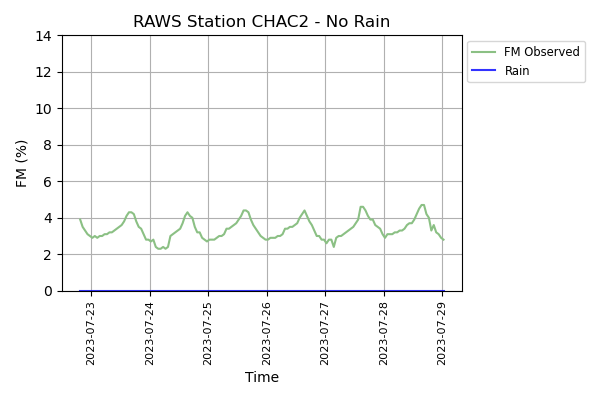
\includegraphics[width=0.8\textwidth]{images/no_rain_plot.png}
    \caption{FMC over time, no rain.}
    \label{fig:fmc_no_rain}
\end{figure}

\begin{figure}[ht]
    \centering
    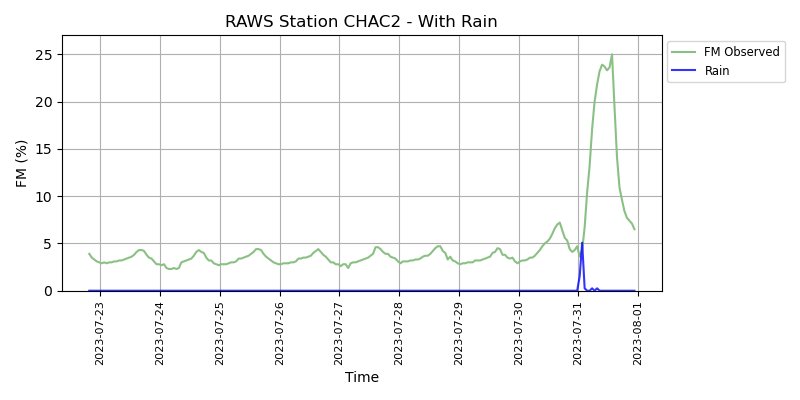
\includegraphics[width=0.8\textwidth]{images/rain_plot.png}
    \caption{FMC over time, with rain.}
    \label{fig:fmc_with_rain}
\end{figure}

Relative humidity and air temperature have a complicated relationship with FMC. Figure \ref{fig:rh_temp_plot} plots the relationship between these two predictors and the FMC at RAWS station CHAC2 for a period of observed values.\footnote{A subset of 1,000 hours of data are plotted for clarity.} The observed correlations in these plots correspond to 0.78 and -0.48, respectively. 

\begin{figure}[ht]
    \centering
    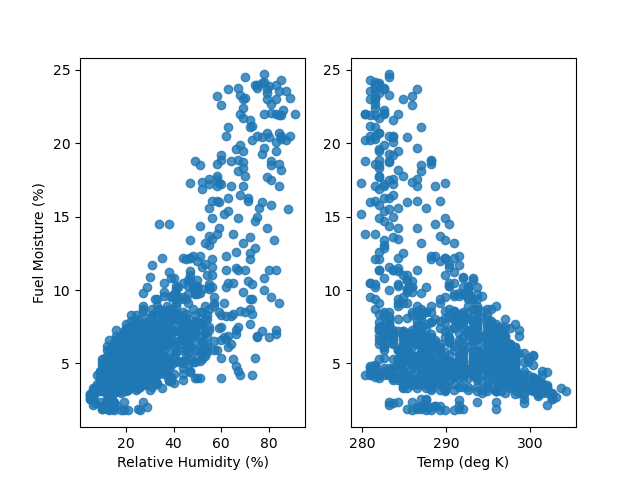
\includegraphics[width=0.8\textwidth]{images/rh_temp_plot.png}
    \caption{RH and Temperature relationship with FMC.}
    \label{fig:rh_temp_plot}
\end{figure}

When relating RH and temperature to equilibrium moisture content using the Equation \ref{eq:equil}, the relationship is much clearer, as can be see in Figure \ref{fig:eq_rh_temp_plot}. The observed correlations in these plots correspond to 0.99 and -0.84, respectively, so the linear relationships are much stronger when using the equilibrium moisture content. Thus, in this project the equilibrium moisture content will be used as a predictor of FMC, rather than using RH and temperature separately.

\begin{figure}[ht]
    \centering
    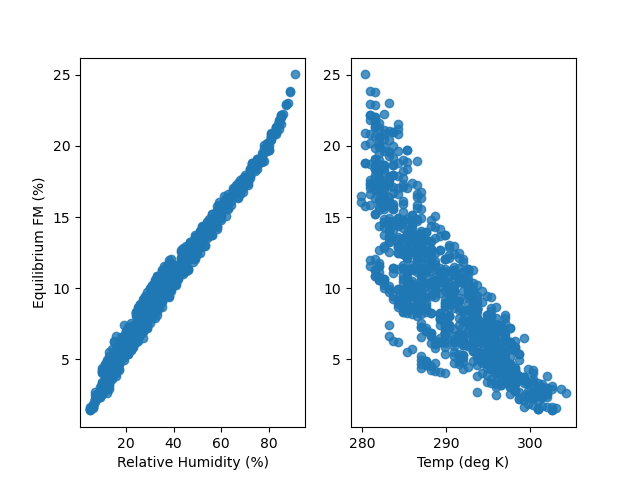
\includegraphics[width=0.8\textwidth]{images/eq_rh_temp_plot.png}
    \caption{RH and Temperature relationship with Drying Equilibrium.}
    \label{fig:eq_rh_temp_plot}
\end{figure}

As discussed previously, the equilibrium moisture content is the theoretical FMC of a piece of wood if kept in constant atmospheric conditions for a long time. The fuel class, e.g. 10-hour fuel, characterizes how quickly the FMC responds to a change in atmospheric conditions. Figure \ref{fig:eq_plot} shows the FMC over time, along with the wetting and drying equilibrium moisture content. Notice how the upward sloping sections of the FMC curve occur slightly later in time than the upward sloping sections of the equilibrium moisture variables. 

\begin{figure}[ht]
    \centering
    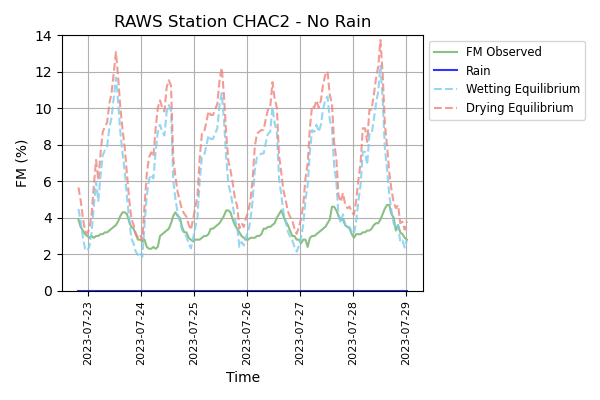
\includegraphics[width=0.8\textwidth]{images/eq_plot.png}
    \caption{FMC \& equilibrium over time.}
    \label{fig:eq_plot}
\end{figure}

\section{Methods}

\subsection{Proposed Loss Functions}

The purpose of the custom loss functions used in this project is to place more weight on model residuals for drier fuels. It is hypothesized that this will lead to more accurate ROS forecasts due to the nonlinear relationship between FMC and ROS, as depicted in Figure \ref{fig:fmc_ros_fmc}. A simple exponentially weighted loss function will be considered. From Equation \ref{eq:wmse}, the weights $w_i$ will be a function of the level of the $i^{th}$ observation of the response variable $y_i$. The weight for the $i^{th}$ residual and corresponding loss function will be:

\begin{equation}
    \label{eq:weights}
    w_i = \exp(-\omega y_i)
\end{equation}

\begin{equation}
    \label{eq:wloss}
    \text{Exponentially Weighted MSE} = \frac{1}{N}\sum_{i=1}^N \exp(-\omega y_i)\cdot (y_i - \hat y_i)^2
\end{equation}

The parameter $\omega$ represents the strength of the weighting scheme relative to an unweighted MSE. When $\omega = 0$, $w_i = 1$ for all $i$, and Equation \ref{eq:wmse} reduces to the standard MSE defined in Equation \ref{eq:mse}. As $\omega$ increases, model residuals associated with larger values of $y_i$ (wetter fuels) are multiplied by a smaller weight and thus contribute less to the overall model loss. Figure \ref{fig:weights} shows the weighting scheme for various values of $\omega$, ranging from $0$ to $0.5$. The line labeled ``Equal Weight" corresponds to the standard MSE and applies a weight of 1 for all residuals in the loss function. The dotted and dashed lines represent the weights used by the exponential weighting schemes. The $\omega$ parameter is the constant in the exponential equation, and as that parameter increases,\footnote{Note the exponential is defined to be negative, so as $\omega$ increases, the exponential has a decreasing negative power.} less weight is given to residuals associated with higher observed values of FMC. The ROS curve is plotted together with these exponential weighting curves for comparison.\footnote{Note: in the right side of Figure \ref{fig:weights}, the ROS curve is rescaled.} 


For this project, the following loss functions will be compared:

\begin{itemize}
    \item The standard MSE.
    \item Exponentially weighted MSE with a grid of 10 different $\omega$ values, ranging from $0.01$ to $0.25$.
    \item A weighted MSE with weights coming from the ROS curve shown in Figure \ref{fig:fmc_ros_fmc}.
\end{itemize}

\begin{figure}[ht]
    \centering
    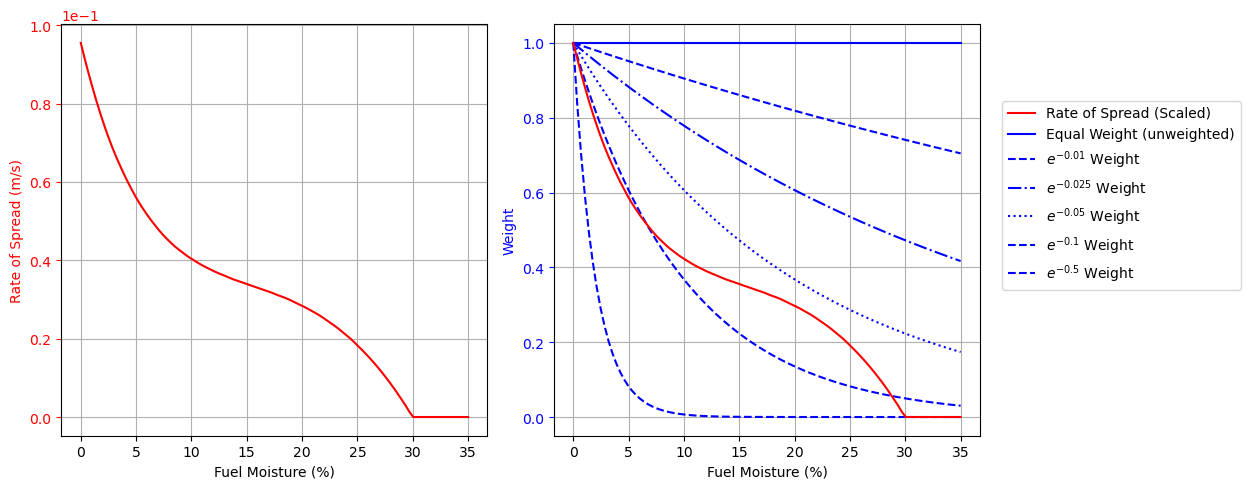
\includegraphics[width=1.1\textwidth]{images/weights.png}
    \caption{Loss Function Weights.}
    \label{fig:weights}
\end{figure}



\subsection{Machine Learning Models}

The goal of this project is to analyze the effect of using the custom loss functions for training machine learning models of FMC. Several different machine learning models will be considered in order to examine whether the custom loss functions have a similar effect across different model architectures. The models used in this project will be linear regression, XGBoost, and Random Forest.\footnote{See Appendix \ref{app:ml} for more information on the models.} These models have been tested by other researchers looking in the FMC modeling literature. \cite{Lee-2020-EFM,McCandless-2020-EWS, Schreck-2023-MLV}

For each model, the same sets of training and testing data will be used. Each model will therefore be modeling the same functional mapping from the predictors at time $t$ to the response variable at time $t$.\footnote{The day of the year of the hour of the day are used as predictors, but this is different from a recursive model like a RNN or an autoregressive model.} Hyperparameter selection is important for machine learning models,\footnote{Hyperparameters in the context of machine learning are fixed parameters that are not updated in the training processes. Adjusting hyperparameters is known as ``tuning", and requires repeatedly training the model and evaluating forecast accuracy.} and in this project a simple manual grid search was conducted. Further research will utilize a more systematic approach to hyperparameter selection. 


\subsection{Model Evaluation}

To evaluate the effects of the various loss functions on the accuracy of ROS forecasts, an experimental setup was constructed where the three machine learning models were trained on a period of data and used to predict the FMC at unobserved times and locations. The FMC predictions were transformed into ROS values for final accuracy metrics. 

\subsubsection{Cross-Validation of Spatiotemporal Models}
\label{sec:cv}

In statistics, cross-validation refers to a set of methods used for evaluating model accuracy on unobserved data.\cite{Hastie-2010-ESL} The data used to fit model parameters is referred to as the ``training set" of data, and the model used to calculate prediction accuracy for the model is referred to as the ``test set" data. It is important that the testing data be independent of the training data. If not, the situation is known as ``data leakage", and this can lead to unreliable estimates of model accuracy.

In the context of FMC modeling, the models are spatiotemporal in nature, or the models predict values at a specific time for a specific location in space. Cross-validation procedures must be formulated carefully to avoid data leakage. The typical approach in machine learning would be to take a random sample of all of the data and hold some portion out to use as a test set. This method would typically lead to data leakage in the spatiotemporal context. To get a meaningful estimate of model accuracy, the test set must consist of observations at locations not included in the training set. Additionally, the test set should be at times in the future compared to all of the training set. 

In this project, the data was split into training and test sets in the following way. Starting with the earliest record of data,\footnote{After data filters, it was the time: May 17, 2023 at 2:22 UTC.} 30 days worth of data used. For those 30 days of data, a random sample of 20\% of the unique locations in the data were selected for inclusion in the test set. Then, the final 2 days of observations in that 30 day period were selected from those locations. So, 80\% of the unique locations of data over 28 days were used to fit model parameters, with observations taken from the start of the period through to 2 days before the end of the period. Then, the fitted model was used to predict FMC at the 20\% of locations that were held out from training, and at times corresponding to the last two days of the period. After that, the 30 period window is moved 2 days into the future. So the second iteration of test data were the 2 days immediately following the previous 2 days test set. In this way, the test sets had no overlap, but the training sets had at most 26 days of overlap. This led to a total of 167 training and testing periods.



\subsection{Loss Function Experimental Design}

Using the data collected from RAWS within the Rocky Mountain GACC, the data was split into training and testing periods using the process described in the previous section. A total of twelve loss functions were considered: the standard MSE, ten weighted schemes with varying $\omega$ parameters, and one with weights determined directly from the ROS transformation of FMC. For each of the twelve loss functions, the three machine learning models described previously were fit to the training set and the fitted model was used to predict new values in the test set. 

The model accuracy is calculated by comparing the predicted FMC in the test set to the observed FMC through the root mean squared error (RMSE). The RMSE is useful since it is interpretable in the same units as the response variable, so a RMSE of 4 can be interpreted as the model having on average a 4\% error in the FMC. This process is repeated 5 times in order to get different random samples of locations to use in the test set. 

For the 167 training and testing periods, 3 machine learning models were fit using 12 different loss functions. Thus, 2,004 RMSE calculations were made for each model, for a total of 6,012 RMSE calculations.

\section{Results}

The results of the analysis described above showed that there was a small reduction in the prediction accuracy for the weighted loss functions.

To compare the RMSE of predictions from the models trained with different loss functions, the different time periods used for training and testing are considered to be independent realizations of the same data generating process. In other words, the RMSE for the various test periods are aggregated to calculate a mean and standard error of the RMSE. Figure \ref{fig:results1} shows the results aggregated over the time periods. The dots represent the mean RMSE, and the vertical line the standard error of the mean RMSE. On the x-axis, the label ``exp\_0.01" corresponds to the exponentially weighted loss function with weight $w_i = \exp(-0.01\cdot y_i)$, where $y_i$ is the $i^{th}$ response value. The vertical dashed line in the plot is meant to distinguish the ROS weighting scheme from the others. The other loss functions are a continuum; the ``MSE" corresponds to an $\omega$ parameter of zero, and then the $\omega$ parameter increases across the x-axis until ``exp\_0.25", which corresponds to $\omega=0.25$. The weighting scheme using the ROS curve is separate from this continuum. The left side of Figure \ref{fig:results1} shows the results of the trained models when predicting the untransformed FMC values. The right side shows the results of the models when predicting the transformed ROS response.

The results for predicting ROS show a U-shaped curve for the weighted loss functions,\footnote{Again, note that the ROS category is not part of this continuum.} where a small amount of weighting of the residuals led to a smaller test RMSE, but when the strength of the weighting scheme increases the accuracy deteriorates. The exponential weighting scheme with $\omega = 0.0367$ resulted in the smallest test RMSE for ROS predictions. These results were small, however, representing just over a 1\% reduction in the RMSE compared to the standard MSE loss function, and the results were not statistically significant.\footnote{A two-sample t-test comparing the RMSE values for the standard MSE loss function and the weighted loss function with $\omega = 0.0367$ resulted in a p-value of roughly 0.54.} Visually this can be seen the the strong overlap between the standard errors of the means.\footnote{The vertical lines representing standard error overlap.} The RMSE using the ROS for weights had similar very similar results to the minimum RMSE results from the $\omega = 0.0367$ weighting scheme. Figure \ref{fig:results2} in Appendix \ref{app:res} shows the results broken down by machine learning model. The pattern is similar for the different models, supporting the idea that conclusions can be drawn about the loss functions themselves.

\begin{figure}[ht]
    \centering
    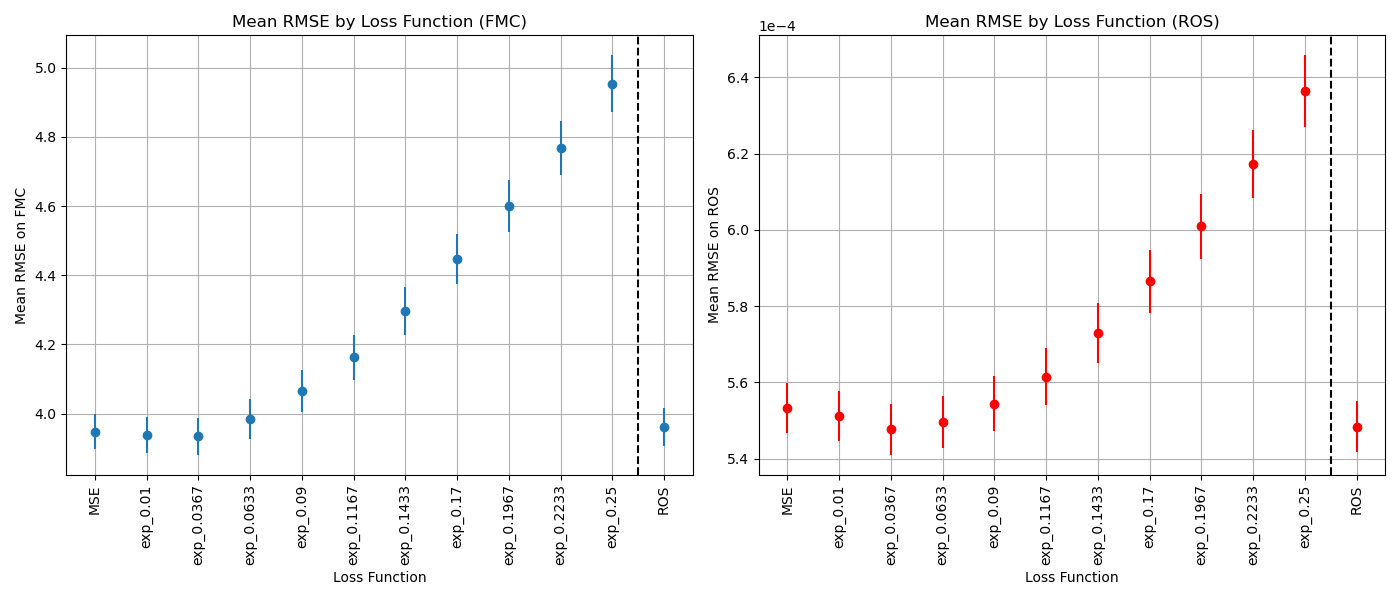
\includegraphics[width=1\textwidth]{images/results1.png}
    \caption{Forecast RMSE Results.}
    \label{fig:results1}
\end{figure}

\section{Discussion}

The results for the RMSE of the FMC values was unexpected. The MSE as a loss function did not result in the lowest MSE in the test set. Using biased estimators by weighting the loss function resulted in slightly lower RMSE on the test set. A hypothesis to explain this relates to the effect of rain. As was shown in Figure \ref{fig:fmc_with_rain}, following rain events the FMC spikes up and then quickly falls back down after the rain passes. These events are relatively rare in the data as there are not long sustained periods of nonzero rain. These spikes in FMC following rain are associated with high levels of FMC, which correspondingly receive less weight when using the weighted loss functions. So, the weighted loss functions may have the effect of downweighting ``outlier" events and causing them to have less of an effect on the model predictions. This finding may show that downweighting FMC observations following rain might lead to an overall more accurate model.

This analysis shows that weighted loss functions can produce at least as accurate results as a standard MSE loss function for machine learning models of FMC, when looking at both the prediction accuracy of FMC itself, and of the transformation to ROS. While it cannot be concluded from this analysis that the weighted loss functions actually improved forecast accuracy for ROS, this analysis provides a hint of a signal that this might be useful if applied to real wildfire simulations. If the estimate of a roughly 1\% reduction in error of ROS were true, that might provide a meaningful improvement in wildfire simulations. This analysis used roughly 1 year of data from the Rocky Mountain region, and a more thorough analysis with data from other time periods and regions of the country could be performed to draw stronger conclusions about the effect of the weighted loss functions.

A number of simplification were used in this analysis. In real-time simulations of wildfires, ROS is a complicated function of local environmental conditions, such as terrain slope. It is not clear how weighted loss functions would perform under more realistic conditions for estimating ROS. The machine learning models used in this report were also not subjected to exhaustive hyperparameter search schemes, and more finely tuned models might interact with the loss functions differently. Additionally, the models used in this report were static, meaning the time dependence of the system was not explicitly modeled. 

Future research could apply the weighting scheme to RNNs or autoregressive models to examine the effect on forecast accuracy. One attractive feature about the weighted loss functions used in this analysis is that they are easy to implement in modern machine learning software packages.\footnote{The neural network software library Tensorflow, for example, has a parameter ``sample\_weight" that easily adds weighting to the standard MSE loss function.} A longer-term goal would be to run multiple real wildfire simulations, using a platform like WRF-SFIRE, with different estimates of FMC produced by models using different loss functions.


\newpage
\bibliographystyle{plain}
\bibliography{ref/fire,ref/fmc,ref/ml}


\appendix
\section{Data Processing} 
\label{app:data}


Calculate Rain from Accumulated
Filter out erroneously high, 100 mm and negative

Calculate equilibrium moisture 
Filter out negatives

Handle NAs
Moisture less than 1 to NA

\hrule

The data retrieval was performed on the University of Colorado Denver computing cluster. The retrieval code exists on github as part of the "wrfxpy" python software package, part of the larger OpenWFM project. The exact python function, which was called with parameters from an executable file, can be found at: \url{https://github.com/openwfm/wrfxpy/blob/develop-72-jh/src/ingest/build_raws_dicts.py}

\subsection*{Data Transformations}

Air temperature observations were converted from Celsius into Kelvin, since the constants in the equations of equilibrium moisture depend on those units. Hourly rainfall, in units of mm/hour, was calculated from the hourly accumulated rainfall by taking the first difference in time. RAWS stations measure hourly accumulated precipitation using a rain gage bucket. These buckets fill up with rain over time and must be occasionally emptied. Some potential sources of error for this data include faulty sensors, uneven rain gage buckets, full rain gages that aren't emptied out when more rain is falling, etc. \cite{campbell} Rainfall observations were filtered out and considered missing if they were over 100mm or less than zero. Additional filters could be explored in future research.

The time of the data observation as retrieved from Synoptic is in Universal Time Coordinated (UTC) format. From this time, the hour of the day, from 0 to 23, is extracted. The hour of the day is used to help the models learn the periodic effect of the diurnal wetting and drying cycles that fuels experience. Humidity and temperature, the main physical drivers of fuel moisture, both have a diurnal pattern of regular highs and lows. These periods correspond with the diurnal pattern of the sun in the sky, where daily maximums in temperature and minimums of humidity occur in the afternoon. A simplifying assumption made in this project is to treat all of these hours the same across a larger geographic region. To make the hour of the day more physically meaningful, the hour would be adjusted based on the position of the sun as it moves in the longitudinal direction. The geographic region in this study is the Rocky Mountain GACC, which spans from central utah through Kansas in the West to East direction. This is a distance of almost 1,500 kilometers. At those distances, there may begin to be meaningful physical difference in the hour of the day for different locations. There exist methods to use the azimuth of the sun to adjust times between locations.



% \section{Spatiotemporal Cross-Validation} \label{app:cv}
\section{Machine Learning Models of FMDA} 
\label{app:ml}

\subsection*{Linear Regression}

The linear regression model used in this project uses the standard form with a constant intercept term, parameters for each predictor variable, and a random error term. As is standard in statistics, the random error is assumed to be normally distributed with zero mean and unknown variance. Let the response value at time $t$ be $y_t$, the number of predictors be $p$, the $i^{th}$ predictor at time $t$ be $x^{(i)}_t$, the $i^{th}$ parameter be $\beta^{(i)}$, and the random error be the  independent (across all $t$) and identically distributed random variable $\epsilon$ with zero mean and unknown variance $\sigma^2$. The model thus has the mathematical form:

\[
y_t = \beta^{(0)} + \sum_{i=1}^p \beta^{(i)} x^{(i)}_t + \epsilon, \qquad \epsilon\sim N(0, \sigma^2)
\]

CITE: ESL Page 44

\subsection*{Tree-based Methods}

In machine learning, ``tree" based models are a type of architecture used for classification or regression tasks where the data is partitioned some number of steps, and the final model output typically uses a simple average of the response variables associated with the data partitions. Regression trees thus produce piecewise-constant outputs.

CITE: ESL page 295

The term ``ensemble" in machine learning refers to using many different models and aggregating them together. There are several motivations for using ensembles, including reducing the variance of the estimator, and across most modeling tasks there are improvements in accuracy when using ensembles as opposed to single trees. There are two popular forms of tree-based ensemble models that are both used in this project: random forests and XGBoost.

\subsubsection*{Random Forest}

Random Forests are a variety of ensemble learner used in both regression and classification tasks. For some predetermined number of trees, a regression tree is built using a bootstrap sample of the training data, subsetted to a random sample of the available predictors. The bootstrapping and random sampling of the predictors used within the model reduces the variance of the estimator. When bootstrap sampling and random feature subsetting is not used, the trees in the ensemble are highly correlated to each other and the model struggles to learn the relationships between the response variable and the predictors. 

CITE: ESL Page 587

\subsubsection*{XGBoost}

Boosting refers to a variety of ensemble learning methods where the individual ensemble members are very simple, so-called ``weak learners", and then an iterative scheme reweights the data on the observations that the weak learners perform poorly on. In the context of regression trees, a simple regression tree is fit to the data in the first iteration. Subsequent iterations re-weight the data associated with observations that have relatively large residuals. 

Extreme gradient boosting, or XGBoost, is an augmentation of gradient boosting that provides computational benefits and additional functionality. Computational benefits of XGBoost relative to standard gradient tree boosting include efficiently handling sparse data with many missing values and support for parallelization. Additional modeling features of XGBoost include regularization of the parameters (i.e. L2 penalty similar to ridge regression).

CITE: ESL Page 337
CITE: https://xgboost.readthedocs.io/




\section{Further Results}
\label{app:res}

A table of summary RMSE values for predicting FMC is found in Table \ref{tab:fmc_results}. The label $exp\_0.01$ corresponds to $\omega=0.01$, and the weight of the $i^{th}$ residual would therefore be $w_i = \exp(-0.01\cdot y_i)$. The weighted loss function with $\omega=0.0367$ had the lowest mean RMSE, but the difference between this and the standard MSE was not statistically significant (p-value of roughly 0.86).

\begin{table}[ht]
\centering
\caption{RMSE Results for predicting FMC.}
\label{tab:fmc_results}
\begin{tabular}{llrrr}
\toprule
 & Loss & Mean & Min & Max \\
\midrule
0 & MSE & 3.948 & 1.857 & 7.480 \\
1 & $\exp\_0.01$ & 3.937 & 1.825 & 7.645 \\
2 & $\exp\_0.0367$ & 3.935 & 1.790 & 8.097 \\
3 & $\exp\_0.0633$ & 3.986 & 1.810 & 8.528 \\
4 & $\exp\_0.09$ & 4.066 & 1.703 & 8.917 \\
5 & $\exp\_0.1167$ & 4.163 & 1.639 & 9.252 \\
6 & $\exp\_0.1433$ & 4.297 & 1.580 & 9.534 \\
7 & $\exp\_0.17$ & 4.448 & 1.583 & 9.853 \\
8 & $\exp\_0.1967$ & 4.601 & 1.546 & 10.276 \\
9 & $\exp\_0.2233$ & 4.767 & 1.507 & 10.636 \\
10 & $\exp\_0.25$ & 4.954 & 1.464 & 11.300 \\
11 & ROS & 3.962 & 1.800 & 8.523 \\
\bottomrule
\end{tabular}
\end{table}

A table of summary RMSE values for predicting ROS is found in Table \ref{tab:ros_results}. The weighted loss function with $\omega=0.0367$ had the lowest mean RMSE, but the difference between this and the standard MSE was not statistically significant (p-value of roughly 0.54).

\begin{table}[ht]
\centering
\caption{RMSE Results for predicting ROS.}
\label{tab:ros_results}
\begin{tabular}{llrrr}
\toprule
\toprule
 & Loss & Mean & Min & Max \\
\midrule
0 & MSE & 5.533e-04 & 2.325e-04 & 1.022e-03 \\
1 & $\exp\_0.01$ & 5.511e-04 & 2.423e-04 & 1.030e-03 \\
2 & $\exp\_0.0367$ & 5.477e-04 & 2.341e-04 & 1.054e-03 \\
3 & $\exp\_0.0633$ & 5.496e-04 & 2.214e-04 & 1.091e-03 \\
4 & $\exp\_0.09$ & 5.544e-04 & 2.165e-04 & 1.128e-03 \\
5 & $\exp\_0.1167$ & 5.615e-04 & 2.177e-04 & 1.182e-03 \\
6 & $\exp\_0.1433$ & 5.730e-04 & 2.138e-04 & 1.197e-03 \\
7 & $\exp\_0.17$ & 5.865e-04 & 2.112e-04 & 1.227e-03 \\
8 & $\exp\_0.1967$ & 6.010e-04 & 2.151e-04 & 1.255e-03 \\
9 & $\exp\_0.2233$ & 6.172e-04 & 2.099e-04 & 1.301e-03 \\
10 & $\exp\_0.25$ & 6.364e-04 & 2.194e-04 & 1.381e-03 \\
11 & ROS & 5.484e-04 & 2.219e-04 & 1.085e-03 \\
\bottomrule
\bottomrule
\end{tabular}
\end{table}

A complete table of results can be found on github at: 

\url{https://github.com/jh-206/Custom-Loss-FMDA}

Figure \ref{fig:results2} shows the RMSE calculations for each of the machine learning models separately.

\begin{figure}[ht]
    \centering
    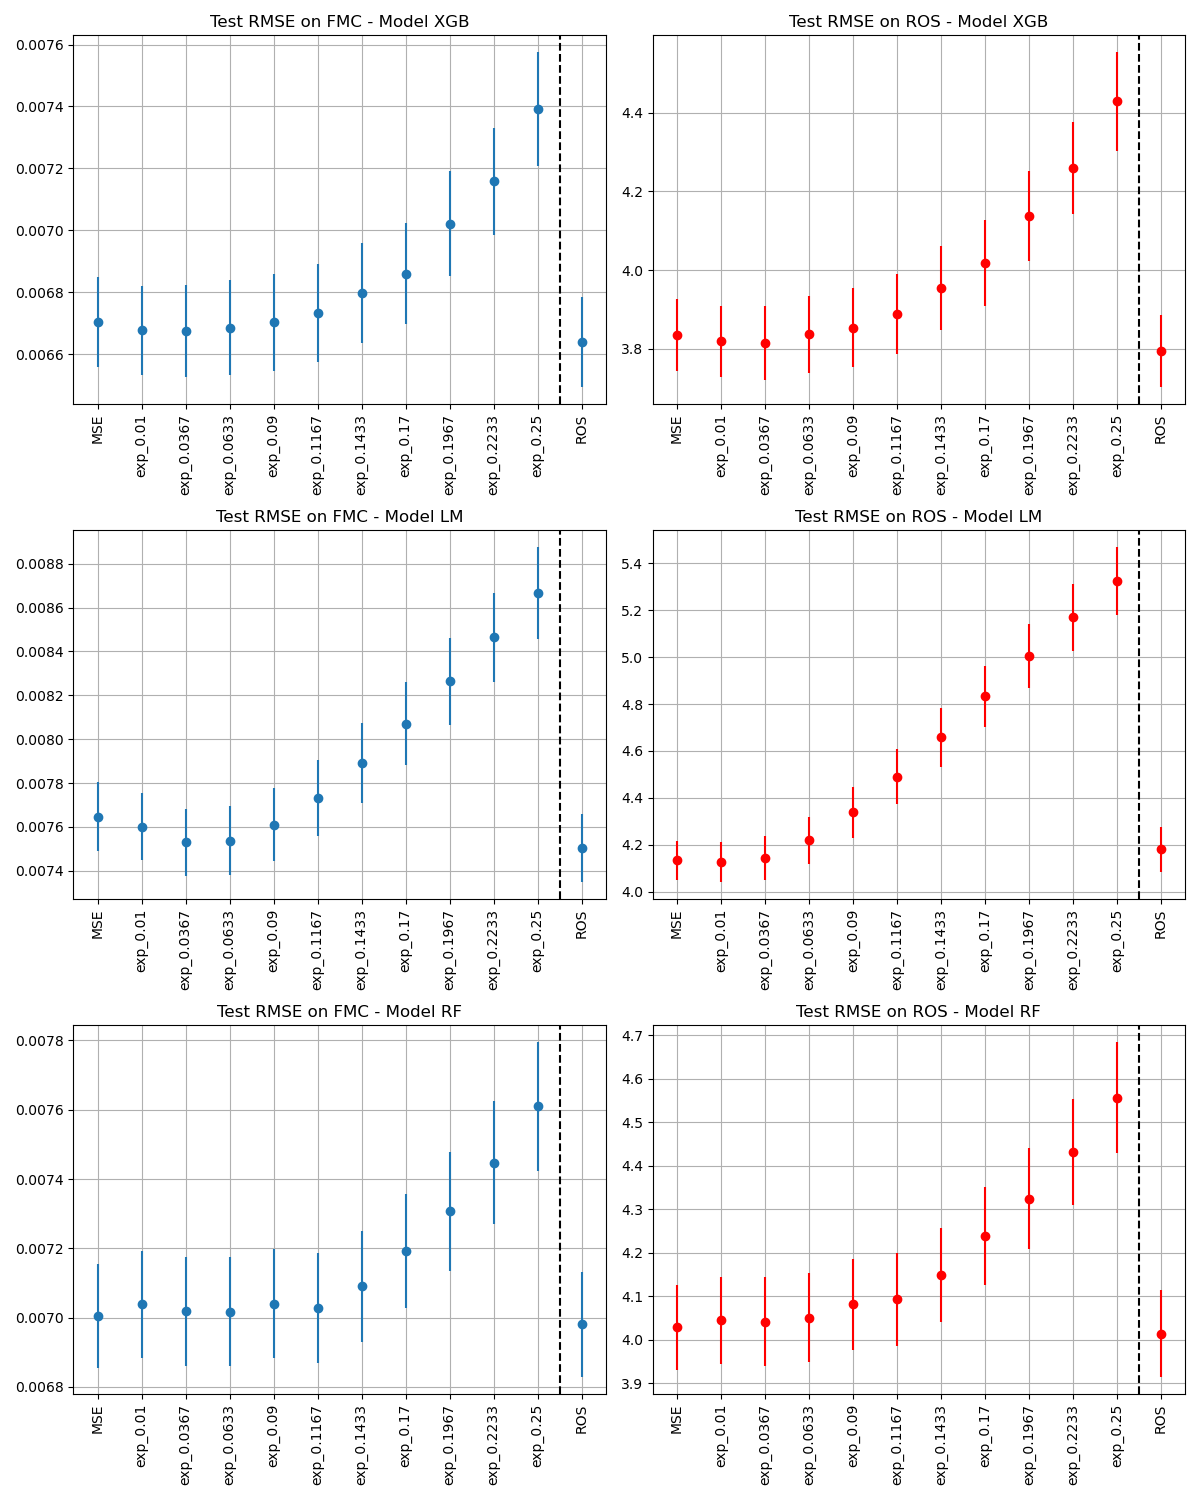
\includegraphics[width=1\textwidth]{images/results2.png}
    \caption{Forecast RMSE Results, by Model.}
    \label{fig:results2}
\end{figure}

\end{document}